\chapter{Concentration and Dilution}\label{ch:g10:concentration-and-dilution}

A hospital drip bag hangs above a patient's bed. Its label reads ``0.9 \%
sodium chloride'': salt in water, nothing more. Yet the figure 0.9 is not
a detail. Too little salt, and the patient's blood cells would swell
with water; too much, and they would shrivel. A solution is not described
by its ingredients alone, but by how much \omterm{def:g6:solutions-and-solubility:solute}{solute} each volume of it
holds, its concentration. This chapter measures concentrations, prepares
solutions of an exact concentration, and dilutes them.

\begin{recall}
A solution is made of a \omterm{def:g6:solutions-and-solubility:solute}{solvent} and one or more dissolved \omterm{def:g6:solutions-and-solubility:solute}{solutes}; the
\omterm{def:g6:solutions-and-solubility:solubility}{solubility} is the largest mass of \omterm{def:g6:solutions-and-solubility:solute}{solute} that a given quantity of
\omterm{def:g6:solutions-and-solubility:solute}{solvent} can \omterm{def:g2:mixing-and-dissolving:dissolve}{dissolve} (\cref{ch:g6:solutions-and-solubility}). The amount
of a species is $n = m/M$, in \omterm{def:g10:the-mole:amount}{moles} (\cref{ch:g10:the-mole}).
\end{recall}

\begin{omfigure}
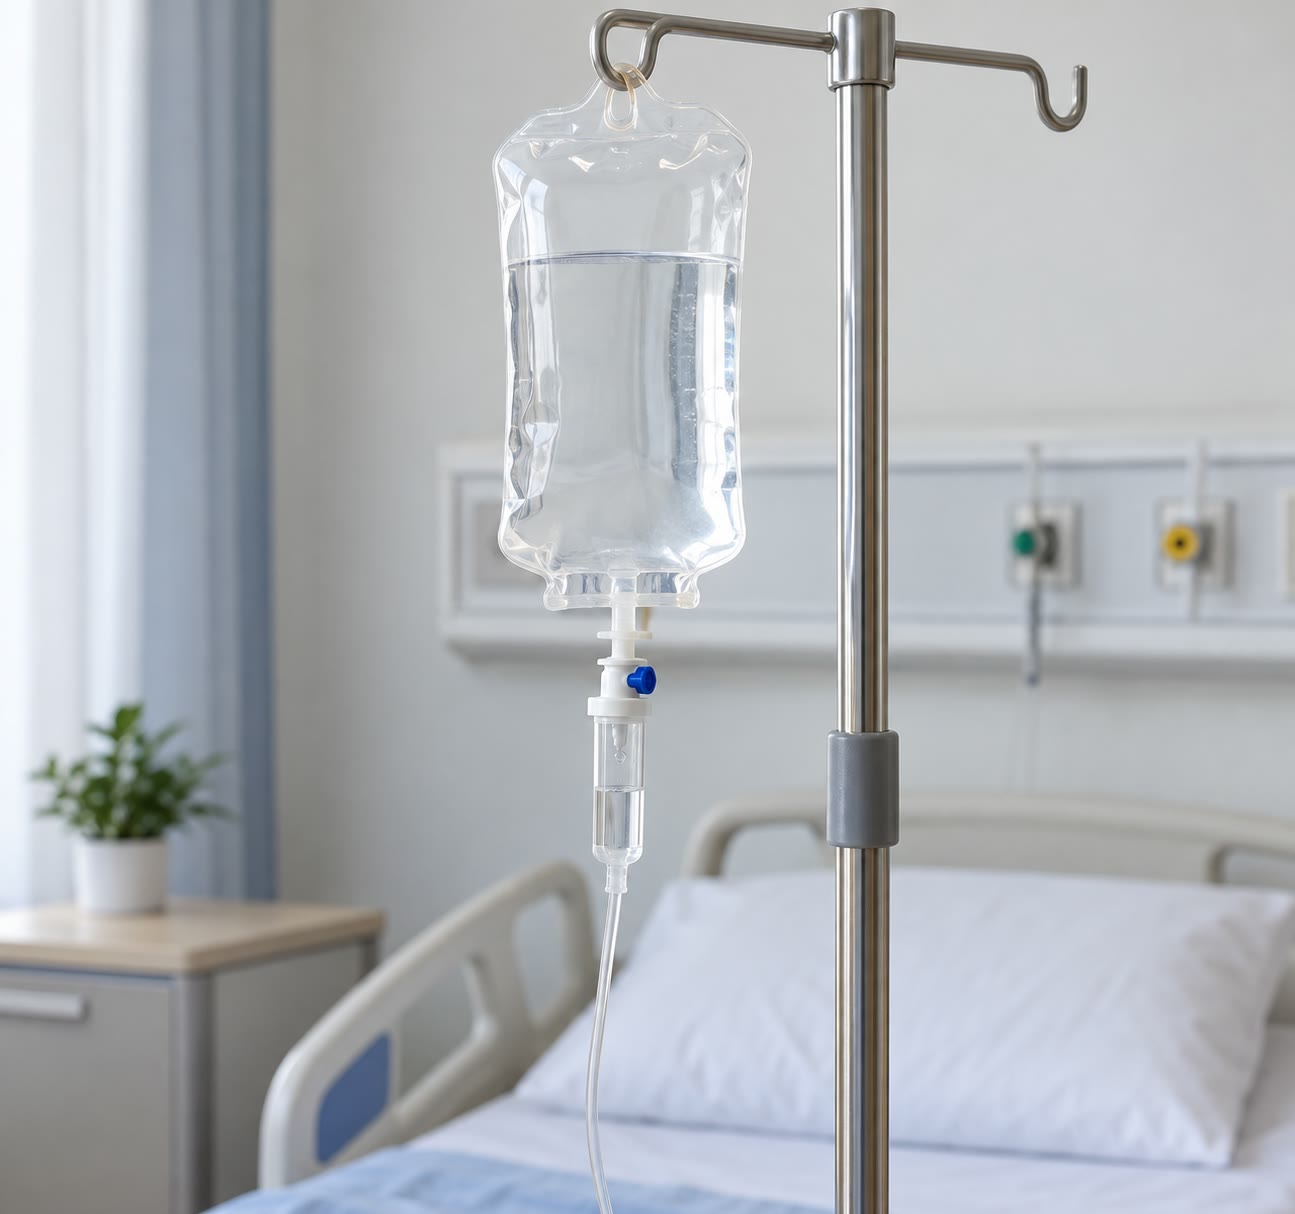
\includegraphics[width=0.42\linewidth]{images/book1/ai/g10-drip-bag.jpg}

{\small A drip bag of salt solution: the concentration must be right.}
\end{omfigure}

\section{Mass concentration}

\begin{definition}[Mass concentration]\label{def:g10:concentration-and-dilution:mass-concentration}
The \emph{mass concentration}\index{mass concentration} $C_m$ of a \omterm{def:g6:solutions-and-solubility:solute}{solute}
in a solution is the mass of dissolved \omterm{def:g6:solutions-and-solubility:solute}{solute} per volume of solution:
\[
  C_m = \frac{m_{\text{solute}}}{V_{\text{solution}}},
\]
in grams per litre (\si{g/L}).
\end{definition}

\begin{example}[Sugared water]\label{ex:g10:concentration-and-dilution:sugar}
\qty{20}{g} of sugar are dissolved in water, and the solution is made up
to \qty{0.50}{L}. Its \omterm{def:g10:concentration-and-dilution:mass-concentration}{mass concentration} in sugar is
$C_m = \qty{20}{g} / \qty{0.50}{L} = \qty{40}{g/L}$. Any part of it has
the same concentration: a glass of \qty{0.20}{L} of it holds
$\qty{40}{g/L} \times \qty{0.20}{L} = \qty{8.0}{g}$ of sugar.
\end{example}


\begin{remark}[The volume is that of the solution]\label{rem:g10:concentration-and-dilution:volume}
The volume in $C_m$ is the volume of the whole solution, not that of the
water poured in: dissolving a \omterm{def:g6:solutions-and-solubility:solute}{solute} changes the volume a little. That
is why a solution is always \emph{made up} to a known final volume, in
a flask marked for it.
\end{remark}

\begin{remark}[Concentration is not solubility]\label{rem:g10:concentration-and-dilution:not-solubility}
% ledger: sol:NaCl, saline:NaCl
The \omterm{def:g6:solutions-and-solubility:solubility}{solubility} of a \omterm{def:g6:solutions-and-solubility:solute}{solute} is the \emph{largest} concentration it can
reach; a solution may have any concentration from zero up to it. Sodium
chloride \omterm{def:g2:mixing-and-dissolving:dissolve}{dissolves} up to about \qty{360}{g} per kilogram of water at
\qty{25}{\celsius}; the drip bag holds only \qty{9}{g} per litre, very
far from saturation.
\end{remark}

\begin{remark}[Percentages on labels]\label{rem:g10:concentration-and-dilution:percent}
% ledger: saline:NaCl
On medical and food labels, ``0.9 \%'' for a solid dissolved in water
usually means \qty{0.9}{g} of \omterm{def:g6:solutions-and-solubility:solute}{solute} per \qty{100}{mL} of solution. In
grams per litre it is ten times more: the drip bag holds \qty{9.0}{g/L}
of sodium chloride.
\end{remark}

\section{Molar concentration}

\begin{definition}[Molar concentration]\label{def:g10:concentration-and-dilution:molar-concentration}
The \emph{molar concentration}\index{molar concentration} $c$ of a
\omterm{def:g6:solutions-and-solubility:solute}{solute} in a solution is the amount of dissolved \omterm{def:g6:solutions-and-solubility:solute}{solute} per volume of
solution:
\[
  c = \frac{n_{\text{solute}}}{V_{\text{solution}}},
\]
in \omterm{def:g10:the-mole:amount}{moles} per litre (\si{mol/L}).
\end{definition}

\begin{proposition}[From one concentration to the other]\label{prop:g10:concentration-and-dilution:link}
For a \omterm{def:g6:solutions-and-solubility:solute}{solute} of \omterm{def:g10:the-mole:molar-mass}{molar mass} $M$,
\[
  C_m = c \times M .
\]
\end{proposition}

\begin{proof}
$C_m = m / V = (n \times M) / V = (n / V) \times M = c \times M$.
\end{proof}

\begin{example}[The drip bag in moles]\label{ex:g10:concentration-and-dilution:drip}
% ledger: saline:NaCl, saline:Na, aw:Na, aw:Cl
The drip bag holds \qty{9.0}{g/L} of sodium chloride, of \omterm{def:g10:the-mole:molar-mass}{molar mass}
\qty{58.5}{g/mol}. Its \omterm{def:g10:concentration-and-dilution:molar-concentration}{molar concentration} is
\[
  c = \frac{C_m}{M} = \frac{\qty{9.0}{g/L}}{\qty{58.5}{g/mol}}
    = \qty{0.154}{mol/L}.
\]
The manufacturer's label gives the same figure the other way round: 154
thousandths of a \omterm{def:g10:the-mole:amount}{mole} of sodium \omterm{def:g9:ions:ion}{ions} per litre.
\end{example}

\begin{remark}[Ions in solution]\label{rem:g10:concentration-and-dilution:ions}
Sodium chloride \omterm{def:g2:mixing-and-dissolving:dissolve}{dissolves} as separate \omterm{def:g9:ions:ion}{ions} \ce{Na+} and \ce{Cl-}
(\cref{ch:g9:ions}): a solution of sodium chloride at \qty{0.154}{mol/L}
holds \qty{0.154}{mol/L} of sodium \omterm{def:g9:ions:ion}{ions} and \qty{0.154}{mol/L} of
chloride \omterm{def:g9:ions:ion}{ions}. How an ionic solid comes apart in water is the subject of
a later chapter.
\end{remark}

\begin{omfigure}
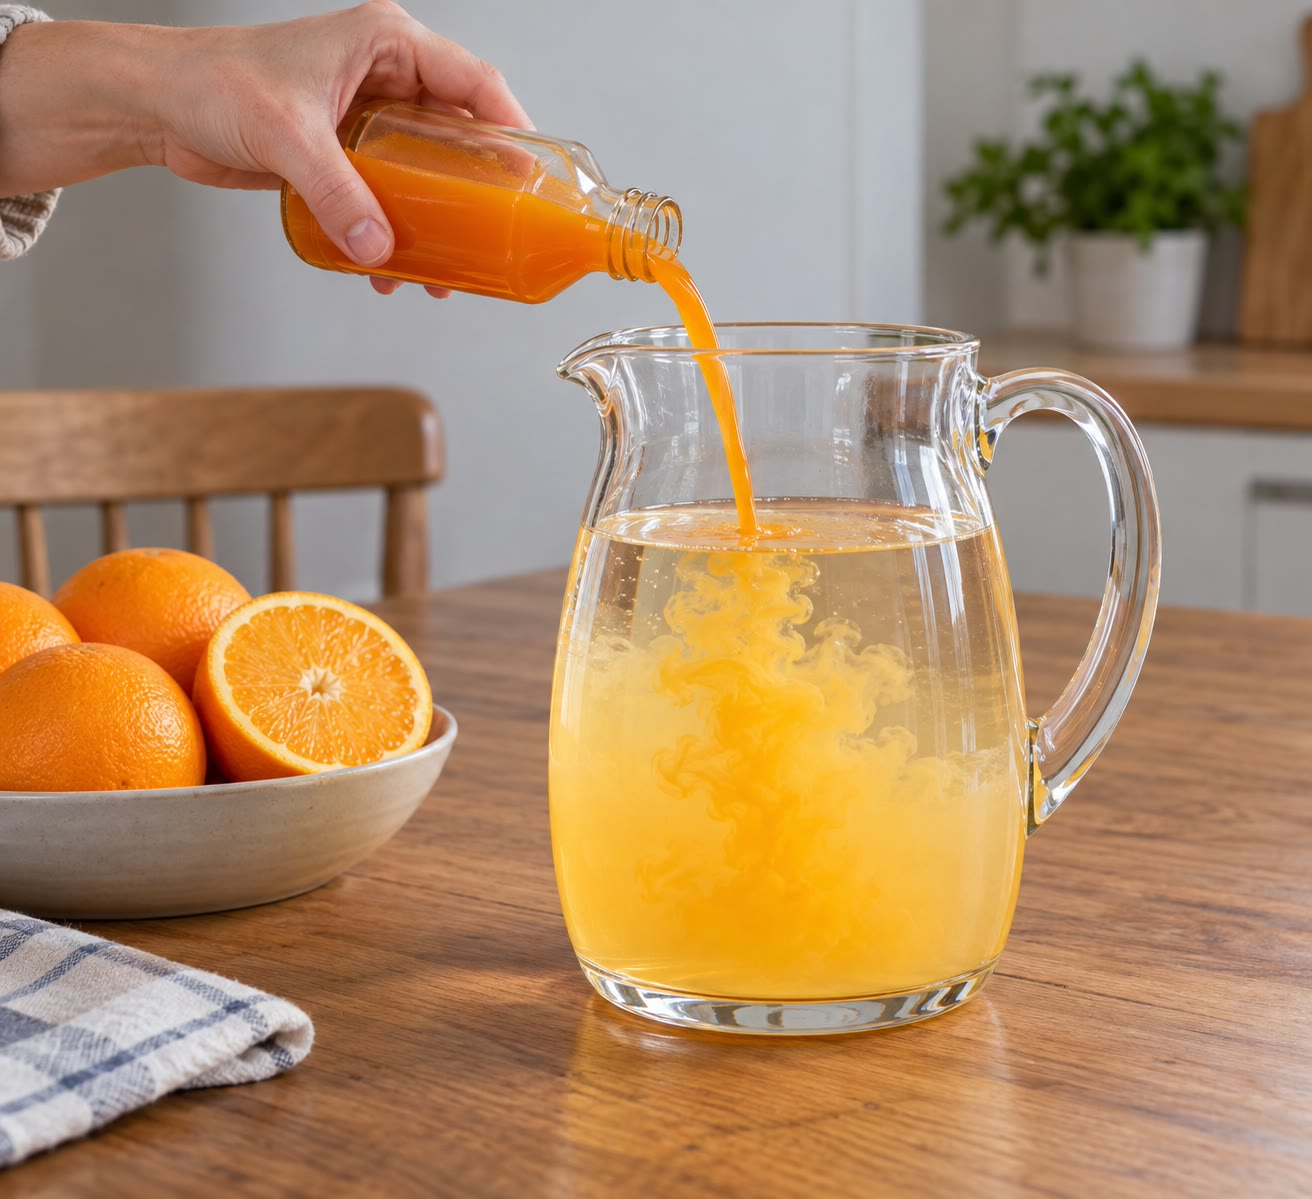
\includegraphics[width=0.45\linewidth]{images/book1/ai/g10-squash-jug.jpg}

{\small Squash from the bottle is diluted with water in a jug: the drink
holds the same amount of fruit syrup, in a larger volume.}
\end{omfigure}

\section{Preparing a solution by dissolving}

\begin{method}[Preparing a solution by dissolving a solid]\label{met:g10:concentration-and-dilution:dissolving}
To prepare a volume $V$ of solution of \omterm{def:g10:concentration-and-dilution:molar-concentration}{molar concentration} $c$:
\begin{enumerate}
  \item Compute the amount needed, $n = c \times V$, and the mass to
        weigh, $m = n \times M$.
  \item Weigh this mass of solid in a small dish on a balance.
  \item Pour the solid through a funnel into a volumetric flask of volume
        $V$; rinse the dish and the funnel with distilled water into the
        flask, so that no solid is lost.
  \item Add distilled water up to about half of the flask and swirl until
        all the solid has dissolved.
  \item Add distilled water up to the mark, the last drops with a dropper;
        stopper the flask and turn it over several times to \omterm{def:g2:mixing-and-dissolving:mix}{mix}.
\end{enumerate}
\end{method}

\begin{omfigure}
\begin{tikzpicture}[font=\small, scale=1.05]
  % 1. weigh
  \pic[transform shape] at (0,0) {balance};
  \fill[black!8, draw=black!55] (-0.45,0.8) -- (0.45,0.8) -- (0.38,0.98)
    -- (-0.38,0.98) -- cycle;
  \fill[white, draw=black!40] (-0.25,0.98) .. controls (-0.1,1.15) and
    (0.1,1.15) .. (0.25,0.98) -- cycle;
  \node[align=center, anchor=north] at (0,-0.2) {1. weigh\\ the solid};
  % 2. transfer through a funnel
  \pic[transform shape] at (3.2,0) {volflask={0.08}{omWater}};
  \pic[transform shape] at (3.2,3.0) {funnel};
  \draw[omProp, thick, -{Stealth}] (2.4,5.0) -- (2.85,4.65);
  \node[align=center, anchor=north] at (3.2,-0.2) {2. transfer,\\ rinse in};
  % 3. half full, swirl
  \pic[transform shape] at (6.4,0) {volflask={0.45}{omWater}};
  \draw[omProp, thick, -{Stealth}] (5.55,0.5) arc[start angle=200,
    end angle=340, x radius=0.9, y radius=0.3];
  \node[align=center, anchor=north] at (6.4,-0.2) {3. half full:\\ swirl to dissolve};
  % 4. to the mark
  \pic[transform shape] at (9.6,0) {volflask={1}{omWater}};
  \fill[black!45] (9.43,3.6) rectangle (9.77,3.85);
  \draw[omDef, thick, <-] (9.82,2.9) -- (10.6,3.3) node[right] {mark};
  \node[align=center, anchor=north] at (9.6,-0.2) {4. fill to the mark,\\
    stopper, mix};
\end{tikzpicture}

{\small Preparing a solution by dissolving a solid: weigh, transfer,
\omterm{def:g2:mixing-and-dissolving:dissolve}{dissolve}, then make up to the mark of the volumetric flask.}
\end{omfigure}

\begin{inthelab}[Filling to the mark]
The mark of a volumetric flask is a ring around its neck. Water in a
narrow glass tube does not end flat: its surface curves down in the
middle, forming a meniscus. The flask is full when the \emph{bottom} of
the meniscus touches the mark, seen with the eye at the level of the
mark, so that the front and the back of the ring look like a single
line. Seen from above or from below, the level can look right when it
is not.
\end{inthelab}

\begin{omfigure}
\begin{tikzpicture}[font=\small]
  \newcommand{\neck}[2]{% x, meniscus bottom height
    \fill[omWater] (#1-0.5,0) -- (#1-0.5,{#2+0.25}) .. controls
      (#1-0.25,#2) and (#1+0.25,#2) .. (#1+0.5,{#2+0.25}) -- (#1+0.5,0) -- cycle;
    \draw[black!60, line width=0.8pt] (#1-0.5,0) -- (#1-0.5,3);
    \draw[black!60, line width=0.8pt] (#1+0.5,0) -- (#1+0.5,3);
    \draw[omDef, line width=0.9pt] (#1-0.5,1.5) -- (#1+0.5,1.5);
    \draw[black!50] (#1-0.5,{#2+0.25}) .. controls (#1-0.25,#2) and
      (#1+0.25,#2) .. (#1+0.5,{#2+0.25});}
  \newcommand{\eye}[2]{% x, y: an eye looking to the right
    \draw[black!70] (#1-0.25,#2) .. controls (#1-0.1,#2+0.18) and
      (#1+0.1,#2+0.18) .. (#1+0.2,#2) .. controls (#1+0.1,#2-0.18) and
      (#1-0.1,#2-0.18) .. (#1-0.25,#2);
    \fill[black!70] (#1+0.05,#2) circle (0.06);}
  % right
  \neck{1.5}{1.5}
  \eye{-0.4}{1.5}
  \draw[dashed, black!50] (-0.1,1.5) -- (2.4,1.5);
  \node[align=center] at (1.5,-0.55) {right: eye level,\\ bottom on the mark};
  % too high
  \neck{6}{1.85}
  \eye{4.1}{1.85}
  \draw[dashed, black!50] (4.4,1.85) -- (6.9,1.85);
  \node[align=center] at (6,-0.55) {too much water:\\ meniscus above};
  % too low
  \neck{10.5}{0.85}
  \eye{8.6}{0.85}
  \draw[dashed, black!50] (8.9,0.85) -- (11.4,0.85);
  \node[align=center] at (10.5,-0.55) {too little water:\\ meniscus below};
\end{tikzpicture}

{\small The neck of a volumetric flask, enlarged and seen with the eye
at the level of the meniscus. The blue line is the mark. Only the
left-hand flask is filled correctly.}
\end{omfigure}

\section{Diluting}

\begin{definition}[Dilution, stock solution, dilution factor]\label{def:g10:concentration-and-dilution:dilution}
A \emph{dilution}\index{dilution} lowers the concentration of a solution
by adding \omterm{def:g6:solutions-and-solubility:solute}{solvent}. The concentrated solution taken at the start is the
\emph{stock solution}\index{stock solution}. The \emph{dilution
factor}\index{dilution factor} $F$ is the ratio of the concentration of
the stock solution to that of the diluted solution:
\[
  F = \frac{c_{\text{stock}}}{c_{\text{diluted}}} .
\]
\end{definition}

\begin{proposition}[The amount of solute is kept]\label{prop:g10:concentration-and-dilution:kept}
During a \omterm{def:g10:concentration-and-dilution:dilution}{dilution}, the amount of \omterm{def:g6:solutions-and-solubility:solute}{solute} does not change: if a volume
$V_0$ of \omterm{def:g10:concentration-and-dilution:dilution}{stock solution} of concentration $c_0$ is made up to a volume
$V_1$, the diluted solution has the concentration $c_1$ given by
\[
  c_0 \times V_0 = c_1 \times V_1,
  \qquad\text{so}\qquad
  F = \frac{c_0}{c_1} = \frac{V_1}{V_0} .
\]
The same holds for \omterm{def:g10:concentration-and-dilution:mass-concentration}{mass concentrations}.
\end{proposition}

\begin{proof}
Only \omterm{def:g6:solutions-and-solubility:solute}{solvent} is added: the \omterm{def:g6:solutions-and-solubility:solute}{solute} taken with the volume $V_0$, an amount
$c_0 V_0$, is all in the final volume $V_1$, where it makes up the
amount $c_1 V_1$.
\end{proof}


\begin{method}[Preparing a solution by dilution]\label{met:g10:concentration-and-dilution:diluting}
To prepare a volume $V_1$ of solution of concentration $c_1$ from a
\omterm{def:g10:concentration-and-dilution:dilution}{stock solution} of concentration $c_0$:
\begin{enumerate}
  \item Compute the volume of \omterm{def:g10:concentration-and-dilution:dilution}{stock solution} to take,
        $V_0 = c_1 V_1 / c_0$ (that is, $V_1 / F$).
  \item Pour a little \omterm{def:g10:concentration-and-dilution:dilution}{stock solution} into a clean beaker (never pipette
        straight from the bottle) and take exactly $V_0$ with a
        volumetric pipette, filled to its mark.
  \item Let the pipette empty into a volumetric flask of volume $V_1$.
  \item Add distilled water up to the mark, stopper and \omterm{def:g2:mixing-and-dissolving:mix}{mix}.
\end{enumerate}
\end{method}

\begin{example}[A tenfold dilution]\label{ex:g10:concentration-and-dilution:tenfold}
A \omterm{def:g10:concentration-and-dilution:dilution}{stock solution} of copper sulfate has $c_0 = \qty{0.10}{mol/L}$;
\qty{100.0}{mL} at $c_1 = \qty{0.010}{mol/L}$ are needed. The \omterm{def:g10:concentration-and-dilution:dilution}{dilution
factor} is $F = 0.10 / 0.010 = 10$, so $V_0 = \qty{100.0}{mL} / 10 =
\qty{10.0}{mL}$: a \qty{10.0}{mL} pipette and a \qty{100.0}{mL} flask.
\end{example}

\begin{omfigure}
\begin{tikzpicture}[font=\small, scale=0.85]
  % 1. take the stock with a pipette
  \pic[transform shape] at (0,0) {beaker={0.6}{cyan!70!blue!55}};
  \pic[transform shape] at (0,0.2) {pipette={1}{cyan!70!blue!55}};
  \node[align=center, anchor=north] at (0,-0.2) {1. pipette $V_0$\\ of stock};
  \draw[omProp, very thick, -{Stealth}] (1.3,2.6) -- (2.6,2.6);
  % 2. empty it into the flask
  \pic[transform shape] at (4,0) {volflask={0.22}{cyan!70!blue!55}};
  \pic[transform shape] at (4,2.6) {pipette={0.12}{cyan!70!blue!55}};
  \node[align=center, anchor=north] at (4,-0.2) {2. empty it into\\ the flask};
  \draw[omProp, very thick, -{Stealth}] (5.3,2.6) -- (6.6,2.6);
  % 3. water to the mark
  \pic[transform shape] at (8,0) {volflask={1}{cyan!70!blue!14}};
  \draw[omDef, thick, <-] (8.2,2.9) -- (9.1,3.4) node[right] {mark};
  \node[align=center, anchor=north] at (8,-0.2) {3. water to the mark:\\
    volume $V_1$};
\end{tikzpicture}

{\small Diluting: a volume $V_0$ of \omterm{def:g10:concentration-and-dilution:dilution}{stock solution}, measured with a
pipette, is made up to $V_1$ in a volumetric flask. The colour fades by
the \omterm{def:g10:concentration-and-dilution:dilution}{dilution factor} $V_1 / V_0$.}
\end{omfigure}

\section{A calibration scale}

\begin{definition}[Standard solution, calibration scale]\label{def:g10:concentration-and-dilution:standard}
A \emph{standard solution}\index{standard solution} is a solution whose
concentration is accurately known. A \emph{calibration
scale}\index{calibration scale} is a series of standard solutions of the
same \omterm{def:g6:solutions-and-solubility:solute}{solute}, at increasing concentrations, usually made by diluting one
\omterm{def:g10:concentration-and-dilution:dilution}{stock solution}; comparing an unknown solution with it gives an estimate
of the unknown's concentration.
\end{definition}

\begin{example}[A blue scale]\label{ex:g10:concentration-and-dilution:scale}
From a \omterm{def:g10:concentration-and-dilution:dilution}{stock solution} of copper sulfate at \qty{0.20}{mol/L}, six
standards are prepared at 0.02, 0.04, 0.06, 0.08, 0.10 and
\qty{0.12}{mol/L}, each in identical tubes filled to the same height.
A solution of unknown concentration, in the same kind of tube, looks
darker than the \qty{0.06}{mol/L} tube and paler than the
\qty{0.08}{mol/L} one: its concentration lies between the two, about
\qty{0.07}{mol/L}.
\end{example}

\begin{omfigure}
\begin{tikzpicture}[font=\small]
  \foreach \i/\c/\p in {0/0.02/8, 1/0.04/16, 2/0.06/24, 3/0.08/32,
                        4/0.10/40, 5/0.12/48} {
    \pic at (1.2*\i,0) {testtube={0.75}{cyan!70!blue!\p}};
    \node[anchor=north] at (1.2*\i,-0.15) {\c};
  }
  \pic at (8.4,0) {testtube={0.75}{cyan!70!blue!28}};
  \node[anchor=north] at (8.4,-0.15) {?};
  \draw[black!40] (7.55,-0.6) -- (7.55,3.2);
  \node[anchor=north] at (3,-0.7) {concentration (\si{mol/L})};
  \node[anchor=north] at (8.4,-0.7) {unknown};
\end{tikzpicture}

{\small A \omterm{def:g10:concentration-and-dilution:standard}{calibration scale} of copper sulfate solutions and an unknown
solution. The unknown lies between the third and fourth tubes.}
\end{omfigure}

\begin{safety}{\ghs[0.82cm]{GHS05}\ghs[0.82cm]{GHS07}\ghs[0.82cm]{GHS09}}
% ledger: ghs:CuSO4
Copper sulfate solutions: harmful if swallowed, irritating to the skin,
damaging to the eyes, very toxic to aquatic life. Goggles and gloves; the
used solutions are collected for treatment, never poured down the sink.
\end{safety}

\begin{remark}[The limits of the eye]\label{rem:g10:concentration-and-dilution:eye}
The eye can only say ``between these two tubes''. To measure a
concentration more finely from the colour of a solution, chemists
measure how much light it absorbs; a later chapter does exactly that.
\end{remark}

\section{Exercises}

\begin{exercise}[$\star$]\label{exo:g10:concentration-and-dilution:1}
\qty{5.0}{g} of sugar are dissolved to make \qty{250}{mL} of solution.
Compute the \omterm{def:g10:concentration-and-dilution:mass-concentration}{mass concentration} of sugar in grams per litre.
\end{exercise}

\begin{exercise}[$\star$]\label{exo:g10:concentration-and-dilution:2}
A solution of \qty{200}{mL} contains \qty{0.050}{mol} of glucose.
Compute its \omterm{def:g10:concentration-and-dilution:molar-concentration}{molar concentration}.
\end{exercise}

\begin{exercise}[$\star$]\label{exo:g10:concentration-and-dilution:3}
What mass of anhydrous copper sulfate \ce{CuSO4} must be weighed to
prepare \qty{100.0}{mL} of solution at \qty{0.10}{mol/L}?
\end{exercise}

\begin{exercise}[$\star$]\label{exo:g10:concentration-and-dilution:4}
A \omterm{def:g10:concentration-and-dilution:dilution}{stock solution} at \qty{1.0}{mol/L} is diluted to \qty{0.050}{mol/L}.
What is the \omterm{def:g10:concentration-and-dilution:dilution}{dilution factor}? What volume of stock is needed to make
\qty{100.0}{mL} of diluted solution?
\end{exercise}

\begin{exercise}[$\star$]\label{exo:g10:concentration-and-dilution:5}
A solution of sodium chloride has a \omterm{def:g10:concentration-and-dilution:molar-concentration}{molar concentration} of
\qty{0.10}{mol/L}. What is its \omterm{def:g10:concentration-and-dilution:mass-concentration}{mass concentration}?
\end{exercise}

\begin{exercise}[$\star\star$]\label{exo:g10:concentration-and-dilution:6}
What volume of a \omterm{def:g10:concentration-and-dilution:dilution}{stock solution} at \qty{0.50}{mol/L} must be taken to
prepare \qty{250.0}{mL} of solution at \qty{0.020}{mol/L}? Name the two
pieces of glassware used.
\end{exercise}

\begin{exercise}[$\star\star$]\label{exo:g10:concentration-and-dilution:7}
Why is a solution of exact concentration made up in a volumetric flask
rather than in a beaker with graduations? Why is a volume of stock
measured with a volumetric pipette rather than with a graduated
cylinder?
\end{exercise}

\begin{exercise}[$\star\star$]\label{exo:g10:concentration-and-dilution:8}
Look at the \omterm{def:g10:concentration-and-dilution:standard}{calibration scale} of copper sulfate. A second unknown is
paler than the \qty{0.04}{mol/L} tube but darker than the
\qty{0.02}{mol/L} one. Estimate its concentration. How could the scale
be changed to estimate it more precisely?
\end{exercise}

\begin{exercise}[$\star\star$]\label{exo:g10:concentration-and-dilution:9}
A glucose solution for infusion contains \qty{50}{g/L} of glucose
\ce{C6H12O6}. Compute its \omterm{def:g10:concentration-and-dilution:molar-concentration}{molar concentration}.
\end{exercise}

\begin{exercise}[$\star\star$]\label{exo:g10:concentration-and-dilution:10}
A syrup is made by dissolving \qty{342}{g} of sucrose \ce{C12H22O11} to
make \qty{1.00}{L} of solution. Compute its \omterm{def:g10:concentration-and-dilution:molar-concentration}{molar concentration}. It is
then diluted ten times. What mass of sucrose does a \qty{20}{mL} spoonful
of the diluted syrup contain?
\end{exercise}

\begin{exercise}[$\star\star$]\label{exo:g10:concentration-and-dilution:11}
A solution has a \omterm{def:g10:concentration-and-dilution:mass-concentration}{mass concentration} of \qty{12}{g/L}. What is its
concentration (a) after water is added to double its volume; (b) after
half of its water has been evaporated, all the \omterm{def:g6:solutions-and-solubility:solute}{solute} remaining
dissolved?
\end{exercise}

\begin{exercise}[$\star\star\star$]\label{exo:g10:concentration-and-dilution:12}
A solution at \qty{0.10}{mol/L} is diluted ten times, the result diluted
ten times again, and once more.
\begin{enumerate}
  \item What is the final concentration?
  \item Why is this done in three steps rather than in a single \omterm{def:g10:concentration-and-dilution:dilution}{dilution}
        by 1000 (think of the volumes of glassware needed)?
\end{enumerate}
\end{exercise}

\begin{exercise}[$\star\star\star$]\label{exo:g10:concentration-and-dilution:13}
\qty{11.1}{g} of calcium chloride \ce{CaCl2} are dissolved to make
\qty{500.0}{mL} of solution. In water the solid separates into calcium
\omterm{def:g9:ions:ion}{ions} \ce{Ca^2+} and chloride \omterm{def:g9:ions:ion}{ions} \ce{Cl-}.
\begin{enumerate}
  \item Compute the \omterm{def:g10:concentration-and-dilution:molar-concentration}{molar concentration} of calcium chloride dissolved.
  \item Deduce the \omterm{def:g10:concentration-and-dilution:molar-concentration}{molar concentrations} of the calcium \omterm{def:g9:ions:ion}{ions} and of the
        chloride \omterm{def:g9:ions:ion}{ions} in the solution.
\end{enumerate}
\end{exercise}

\begin{exercise}[$\star\star\star$]\label{exo:g10:concentration-and-dilution:14}
A \qty{100.0}{mL} volumetric flask has a neck of inner diameter
\qty{1.2}{cm}. A student fills it with the bottom of the meniscus
\qty{2}{mm} above the mark.
\begin{enumerate}
  \item What extra volume of water has been added (volume of a cylinder:
        $\pi r^2 h$)?
  \item By what percentage is the concentration of the solution too low?
\end{enumerate}
\end{exercise}

\begin{exercise}[$\star\star\star$]\label{exo:g10:concentration-and-dilution:15}
\qty{100}{mL} of sodium chloride solution at \qty{0.20}{mol/L} are mixed
with \qty{300}{mL} of sodium chloride solution at \qty{0.10}{mol/L}.
Assuming the volumes add, compute the concentration of the \omterm{def:g6:pure-substances-and-mixtures:mixture}{mixture}. Is
it the average of the two concentrations? Explain.
\end{exercise}

\section{Problem: The Drip Bag}

\begin{problem}[{Weekend problem --- how much of a concentrated salt
solution goes into one bag of ``0.9 \%'' saline?}]
\label{pb:g10:concentration-and-dilution:1}
% ledger: saline:NaCl, saline:Na, sol:NaCl, aw:Na, aw:Cl, const:NA
A hospital pharmacy laboratory keeps a concentrated sterile solution of
sodium chloride containing \qty{200}{g/L} (on its label: ``20 \%''). It
must prepare bags of \qty{500}{mL} of the ``0.9 \%'' solution used in
drips, by diluting the concentrated solution with sterile water.

\medskip
\noindent\textbf{Part I --- What 0.9 \% means.}
\begin{enumerate}
  \item The label ``0.9 \%'' means \qty{0.9}{g} of salt per \qty{100}{mL}
        of solution. Give the \omterm{def:g10:concentration-and-dilution:mass-concentration}{mass concentration} in \si{g/L}.
  \item Express it also in milligrams per millilitre.
  \item What mass of sodium chloride does a \qty{500}{mL} bag contain?
  \item Sodium chloride \omterm{def:g2:mixing-and-dissolving:dissolve}{dissolves} up to about \qty{360}{g} per kilogram
        of water. Is the solution of the bag far from saturation?
  \item A patient receives \qty{1.0}{L} of this solution in a day. What
        mass of salt is that?
\end{enumerate}

\medskip
\noindent\textbf{Part II --- In \omterm{def:g10:the-mole:amount}{moles}.}
\begin{enumerate}[resume]
  \item Compute the \omterm{def:g10:the-mole:molar-mass}{molar mass} of sodium chloride.
  \item Compute the \omterm{def:g10:concentration-and-dilution:molar-concentration}{molar concentration} of the solution of the bag.
  \item What amount of sodium chloride does one bag contain?
  \item What are the \omterm{def:g10:concentration-and-dilution:molar-concentration}{molar concentrations} of sodium \omterm{def:g9:ions:ion}{ions} and of chloride
        \omterm{def:g9:ions:ion}{ions} in the bag?
  \item How many sodium \omterm{def:g9:ions:ion}{ions} does one bag contain?
\end{enumerate}

\medskip
\noindent\textbf{Part III --- From the concentrated solution.}
\begin{enumerate}[resume]
  \item Compute the \omterm{def:g10:concentration-and-dilution:dilution}{dilution factor} between the concentrated solution and
        the solution of the bag.
  \item Which mass of sodium chloride must come from the concentrated
        solution for one bag? Deduce the volume of concentrated solution
        to take.
  \item Check this volume with the \omterm{def:g10:concentration-and-dilution:dilution}{dilution factor}.
  \item Compute the \omterm{def:g10:concentration-and-dilution:molar-concentration}{molar concentration} of the concentrated solution, and
        check that $c_0 V_0 = c_1 V_1$.
  \item About what volume of sterile water is then added (assume the
        volumes add)?
\end{enumerate}

\medskip
\noindent\textbf{Part IV --- Glassware and accuracy.}
\begin{enumerate}[resume]
  \item No volumetric pipette of this volume exists. Which piece of
        glassware, graduated in tenths of a millilitre, could deliver
        it?
  \item In which vessel should the final volume be made up, to be
        accurate?
  \item If \qty{23.0}{mL} were taken instead of the right volume, what
        \omterm{def:g10:concentration-and-dilution:mass-concentration}{mass concentration} would the bag have? By what percentage would
        it be wrong?
  \item State the final answer: what volume of the concentrated
        solution goes into one \qty{500}{mL} bag?
\end{enumerate}
\end{problem}
